\chapter{Experiments}
\label{chap:experiments}

In this chapter the experiments and experimental results of this work are displayed. First we establish the general experimental setup. Afterwards the results of the conducted MVTecAD LOCO \cite{LOCODentsAndScratchesBergmann2022}
survey are presented in section \ref{sec:locoxperiments}. As a baseline for performance evaluation we uitilize the performance on the more conventional MVTecAD dataset \cite{MVTEC_Bergmann_2021}, 
as well as a classifier comparison. In section \ref{sec:faltconnectorxperiments} we review the performance of the classifiers on our novel dataset category. Lastly section \ref{sec:ensembleresults} 
deals with the findings regarding the ensemble network approach, also conducted on the MVTecAD LOCO dataset.


\section{Experimental Setup}
\label{sec:experimentsetup}

All models trainings and result reproductions have been conducted on the IAD cluster student partition. The GPU in use for all nodes used by that partition (ist die formulierung gut?) is and 
RTX 2080Ti with 11GB of memory, and the CPU is an AMD Ryzen 9 16-Core processor. The cluster overview \cite{clusterdocs} serves to provide further detail for additional questions. As for software, 
pytorch 2.1.2 was utilized to implement the ensemble model. The specifications of other libraries, as well as the specifications for the MVTecAD LOCO experiment are documented in the 
environment files in the project code.



\section{MVTecAD LOCO Experiments}
\label{sec:locoxperiments}
In this section we review the performance of prior introduced anomaly detection methods. All experiments were performed with the same 
conditions explained in section (referenz von methods section über loco) 
and on the MVTecAD LOCO dataset \cite{LOCODentsAndScratchesBergmann2022}. 
The results of inference on the test set can be seen in table x (tabelle mit ergebnissen). As it can be seen, all models scored a significantly 
lower result on the MVTecAD LOCO dataset than on the normal MVTecAD one(exemplary scores seen in table xy(table mit normalen mvtec scores)). 
A lower performance is generally to be expected, since firstly logial anomalies are regarded as a more difficult problem than structual 
ones and secondly the average SOTA performances as seen in table x(tabelle mit ergebnissen) is already closing in on an AUROC of of 1. 
(den satz rechts von hier müsste man maybe rausmachen oder umschreiben)Therefore there is not much room for further improvement in similar settings, and a worse performance still aknowledgeable as very good. 
Yet there is an drop in cross-model average AUROC of approcimately (durchschnitts drop ausrechnen), which is a remarkable(synonym) difference. 
Most other metrics, namely (metrics names), also declined with an respective average of (respective averages). As explained in section 
(referenz zu metrics section von background), the sPRO (or rather AU-sPRO) was a score introduced in \cite{LOCODentsAndScratchesBergmann2022} to gain an 
advanced insight on the quality of segmentations. This means that all approaches who either were published before or did not include this 
paper in their research likely did not include this metric, which holds true for the approahces used for this experiment. Therefore no comparison 
in sPRO/AU-sPRO can be shown(vllt einfach spro auch für allte ansätze implementieren?? dann kann ich den satz ändern). Comparing the sPRO 
scores of the SOTA methods in this experiment with the ones from compared to GCAD \cite{LOCODentsAndScratchesBergmann2022} shows asignificantly 
(abchecken ob wirklich) worse performance.
Among the different models, the highest scoring one was PatchCore \cite{patchCore2022}. It scored an average (metrics einfügen) feature embedding based approaches like  
achieved the highest scoring

Interpretation of results hier, weiß nicht in welche section das eigentlich muss:

\begin{figure}[htbp]
    \captionsetup[subfigure]{justification=centering}
    \centering
    \begin{subfigure}[b]{0.3\textwidth}
        \centering
        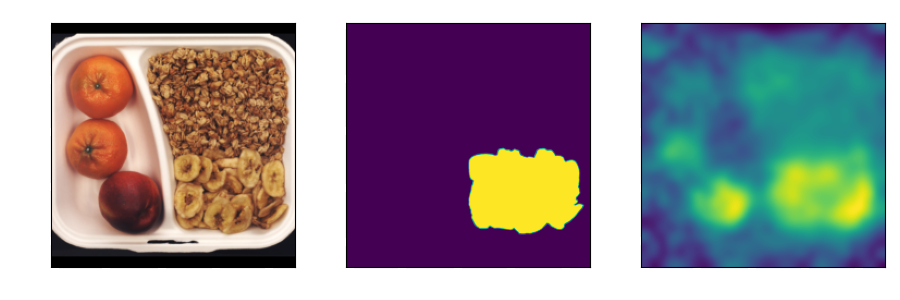
\includegraphics[width=\textwidth]{figures/locopatchcoreresults/breakfast_box_test_logical_anomalies_003.png}
        %\caption*{Logical Anomalies}

    \end{subfigure}
    \begin{subfigure}[b]{0.3\textwidth}
        \centering
        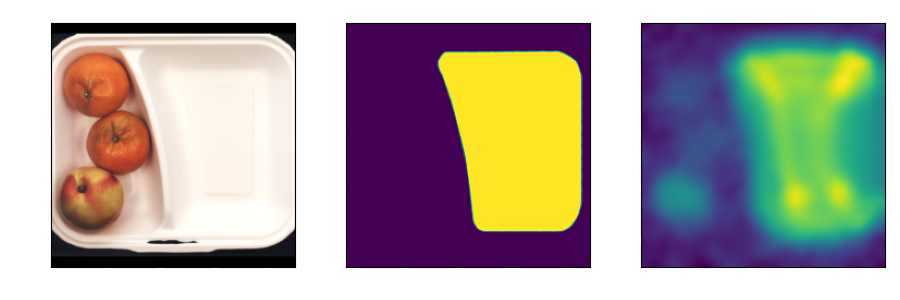
\includegraphics[width=\textwidth]{figures/locopatchcoreresults/breakfast_box_test_logical_anomalies_034.png}


    \end{subfigure}
    \begin{subfigure}[b]{0.3\textwidth}
        \centering
        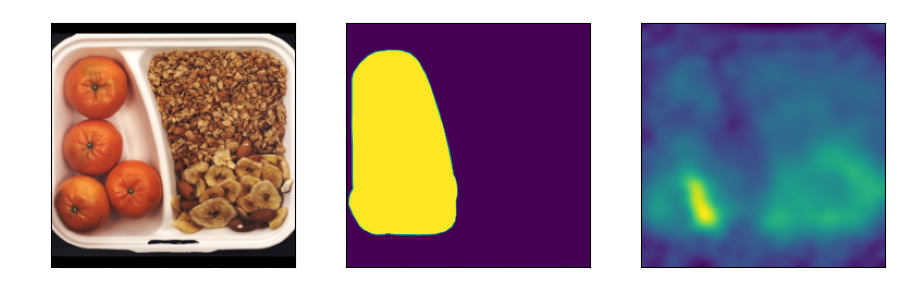
\includegraphics[width=\textwidth]{figures/locopatchcoreresults/breakfast_box_test_logical_anomalies_070.png}


    \end{subfigure}
    \begin{subfigure}[b]{0.3\textwidth}
        \centering
        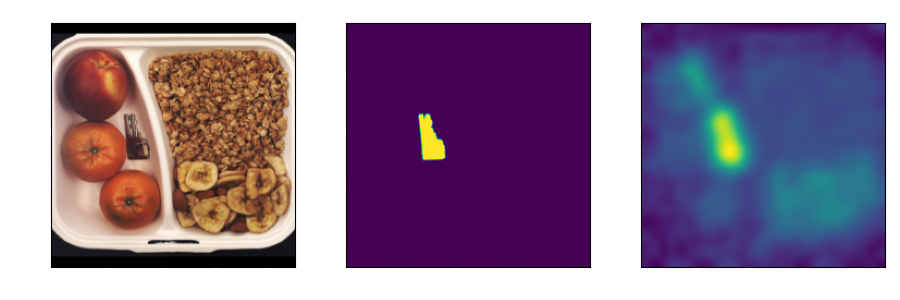
\includegraphics[width=\textwidth]{figures/locopatchcoreresults/breakfast_box_test_structural_anomalies_014.png}
        %\caption*{Structural Anomalies}

    \end{subfigure}
    \begin{subfigure}[b]{0.3\textwidth}
        \centering
        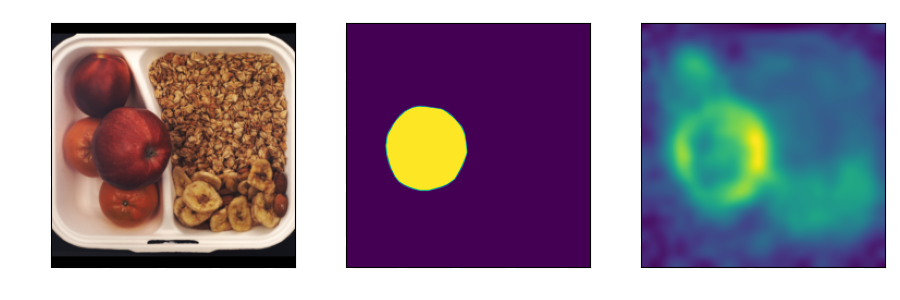
\includegraphics[width=\textwidth]{figures/locopatchcoreresults/breakfast_box_test_structural_anomalies_024.png}


    \end{subfigure}
    \begin{subfigure}[b]{0.3\textwidth}
        \centering
        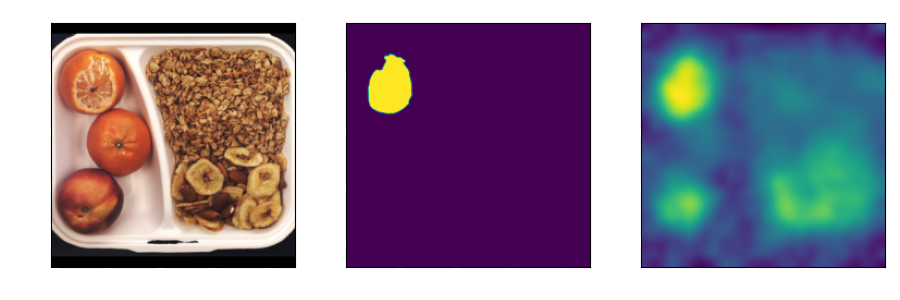
\includegraphics[width=\textwidth]{figures/locopatchcoreresults/breakfast_box_test_structural_anomalies_070.png}


    \end{subfigure}
    \caption{Exemplary Results of PatchCore on the Breakfast Box Class}
    \label{fig:PCBB}
\end{figure}

\section{Flat Connector Experiments}
\label{sec:faltconnectorxperiments}


\section{Ensemble Network}
\label{sec:ensembleresults}

This section reports the results of the ensemble network approach on the class flat connector %austauchen? 
as a flagship experiment for the rest of the dataset. More results from other classes of the MVTecAD LOCO \cite{LOCODentsAndScratchesBergmann2022} set are to be found in appendix (referenz). All conclusions drawn from this 
experiment are also applicable to the other classes. Firstly the results from the primary ensemble approach from section \ref{sec:featurelevelensemble} are reported. Afterwards 
the results of the secondary ensemble approach are presented, supported by according metrics and segmentation examples.


\subsection{Independent Transformation Block}
\label{subsec:ITBfail}

When performing the ensemble training process using the approach by \cite{EnsembleHeller2023}, the results were generally not usable. Looking at the exemplary plot of the segmentation 
results in figure \ref{fig:pca_res}, it becomes obvious why no metrics are reported for this experiment. When investigating image level metrics, they were highly inconsistent thorughout 
the training process and are regarded as not meaningful and representative.

\begin{figure}[htbp]
    \captionsetup[subfigure]{justification=centering}
    \centering
    \begin{subfigure}[b]{0.3\textwidth}
        \centering
        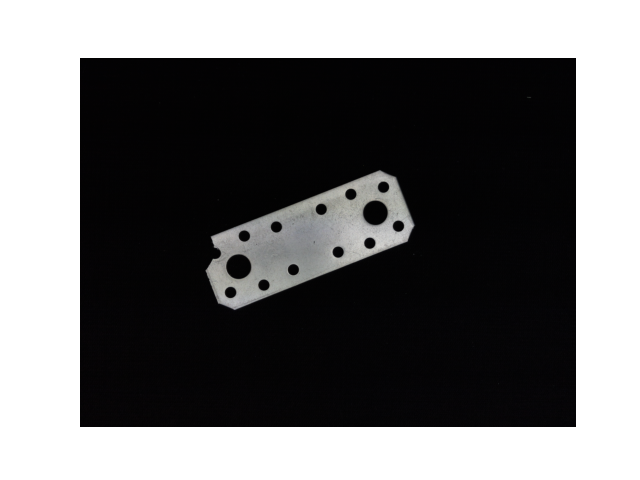
\includegraphics[width=\textwidth]{figures/pca_results/cut_corner.png}
        \caption*{original Image}

    \end{subfigure}
    \begin{subfigure}[b]{0.3\textwidth}
        \centering
        
\includegraphics[width=\textwidth]{figures/pca_results/cut_corner_mask.png}
        \caption*{Mask}

    \end{subfigure}
    \begin{subfigure}[b]{0.3\textwidth}
        \centering
        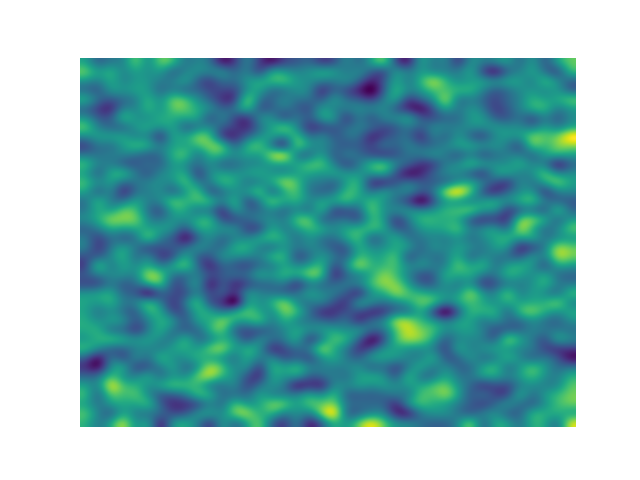
\includegraphics[width=\textwidth]{figures/pca_results/pca_res.png}
        \caption*{Discriminator Predictions}

    \end{subfigure}
    \caption{Results of Independent Transformation Block Ensembles Section \ref{sec:featurelevelensemble}}
    \label{fig:pca_res}
\end{figure}

As visible in figure \ref{fig:pca_res}, the segmentation results appeared to be not more meaningful than gaussian noise, strongly suggesting that this method has failed. Subsection 
\ref{subsec:ITBfaildiscussion} will go into possible reasons for the suboptimal experiments results. Concludingly it is to be said that these results are, besides the failure analysis 
in the conclusion, not relevant and will not be part of further review. Thus no results of other classes using this method are posted in the appendix.

\subsection{Stacking Ensemble}
\label{subsec:stacking}


